%\documentclass{article}
%\usepackage{graphicx,subfigure}
%\begin{document}

\begin{figure}[!h]
  \centering
   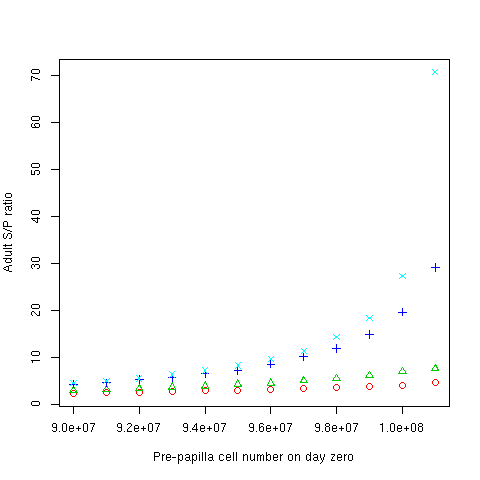
\includegraphics[width=0.9\textwidth]{zcellnosop.png}
  \caption{Calculated values of adult follicle S/P ratio at a range of values of the parameter $(C_{n})_{0}$  from equations ~\ref{eqn:prim} to ~\ref{eqn:sd3} with values for the other 19  parameters fixed at the values given in Table~\ref{tab:base}. The four sets of points correspond to four values of the parameter $C_{b}$, red=.070, green=.073, blue=.076, cyan=.0764, the last being the base value for this cell birth probability parameter}
  \label{fig:zcellnosop}
\end{figure}

%\end{document}

